\documentclass{article}
    
    
    \usepackage{graphicx} % Used to insert images
    \usepackage{adjustbox} % Used to constrain images to a maximum size 
    \usepackage{color} % Allow colors to be defined
    \usepackage{enumerate} % Needed for markdown enumerations to work
    \usepackage{geometry} % Used to adjust the document margins
    \usepackage{amsmath} % Equations
    \usepackage{amssymb} % Equations
    \usepackage{eurosym} % defines \euro
    \usepackage[mathletters]{ucs} % Extended unicode (utf-8) support
    \usepackage[utf8x]{inputenc} % Allow utf-8 characters in the tex document
    \usepackage{fancyvrb} % verbatim replacement that allows latex
    \usepackage{grffile} % extends the file name processing of package graphics 
                         % to support a larger range 
    % The hyperref package gives us a pdf with properly built
    % internal navigation ('pdf bookmarks' for the table of contents,
    % internal cross-reference links, web links for URLs, etc.)
    \usepackage{hyperref}
    \usepackage{longtable} % longtable support required by pandoc >1.10
    \usepackage{booktabs}  % table support for pandoc > 1.12.2
    \usepackage{indentfirst}
    \usepackage{floatrow}
    \usepackage{relsize}
    
    \newcommand\perm[2]{{}_{#1}P_{#2}}%
    
    
    \title{Homework 4}
    \author{Roly Vicar\'ia \\ STAT414 Spring 2016}
    
\begin{document}
    
    \maketitle
    
    Section 2.1
    \begin{enumerate}
     
     \addtocounter{enumi}{2}
     
     %3
     \item 
      \begin{enumerate}
       %a
       \item 
	  We set the sum of $f(x)$ over all $x$ equal to 1,  
	  \begin{align*}
	  1 &= \dfrac{1}{c} + \dfrac{2}{c} + \dfrac{3}{c} + \dfrac{4}{c} \\
	    &= \dfrac{10}{c} 
	  \end{align*}
	  
	  Therefore, $c = 10$.
	  
	  \begin{figure}[h!]
	    \centering
	    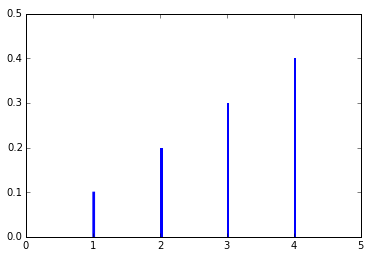
\includegraphics[scale=.5]{./images/3a_pmf-line_graph.png}
	    % 3a_pmf-line_graph.png: 375x256 pixel, 96dpi, 9.92x6.77 cm, bb=0 0 281 192
	  \end{figure}
	
	%b
	\item 
	  $1 = \mathlarger{\sum}_{x=1}^{10}{cx} = 1c + 2c + 3c + \cdots + 10c = 55c$ \\
	  Therefore, $c = \dfrac{1}{55}$
	  
	  \begin{figure}[h!]
	    \centering
	    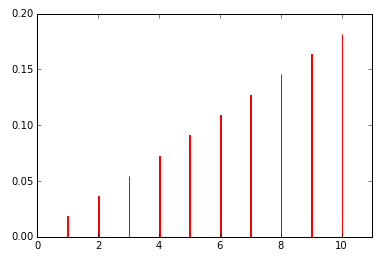
\includegraphics[scale=.5]{./images/3b_pmf-line_graph.png}
	    % 3b_pmf-line_graph.png: 388x256 pixel, 96dpi, 10.26x6.77 cm, bb=0 0 291 192
	  \end{figure}

	%c
	\item 
	  \begin{align*}
	    1 &= \mathlarger{\sum}_{x=1}^\infty{c\left(\dfrac{1}{4}\right)^x} \\
	      &= c \mathlarger{\sum}_{x=1}^\infty{\left(\dfrac{1}{4}\right)^x} \\
	      &= c \left[ \dfrac{1}{4} + \dfrac{1}{4^2} + \dfrac{1}{4^3} + \cdots \right] \\
	      &= c \left[\dfrac{\dfrac{1}{4}}{1 - \dfrac{1}{4}}\right] \\
	      &= c \left( \dfrac{1}{3} \right)
	  \end{align*}
	  
	  Therefore, $c = 3$.
	  
	  \begin{figure}[h!]
	    \centering
	    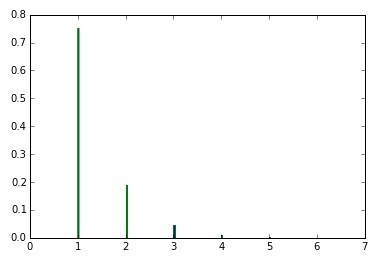
\includegraphics[scale=.6]{./images/3c_pmf-line_graph.png}
	    % 3c_pmf-line_graph.png: 381x256 pixel, 96dpi, 10.08x6.77 cm, bb=0 0 286 192
	  \end{figure}
	  
	%d
	\item
	  \begin{align*}
	    1 &= \mathlarger{\sum}_{x = 0}^3{c(x+1)^2} \\
	      &= c \mathlarger{\sum}_{x = 0}^3{(x+1)^2} \\
	      &= c \left[ (0+1)^2 + (1+1)^2 + (2+1)^2 + (3+1)^2 \right] \\
	      &= c \left[ 1 + 4 + 9 + 16 \right] \\
	      &= 30c
	  \end{align*}
	  
	  Therefore, $c = \dfrac{1}{30}$.
	  
	  \begin{figure}[h!]
	    \centering
	    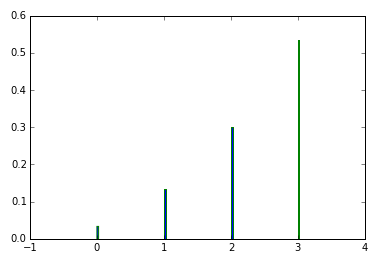
\includegraphics[scale=.6]{./images/3d_pmf-line_graph.png}
	    % 3d_pmf-line_graph.png: 380x258 pixel, 96dpi, 10.05x6.83 cm, bb=0 0 285 193
	  \end{figure}

	  
	%e
	\item
	  \begin{align*}
	    1 &= \mathlarger{\sum}_{x=1}^n{\dfrac{x}{c}} \\
	      &= \dfrac{1}{c} \mathlarger{\sum}_{x=1}^n{x} \\
	      &= \dfrac{1}{c} ( 1 + 2 + \cdots + n ) \\
	      &= \dfrac{1}{c} \cdot \dfrac{n(n+1)}{2} 
	  \end{align*}
	  
	  Therefore, $c = \dfrac{n(n+1)}{2}$.
	  
	  \begin{figure}[h!]
	    \centering
	    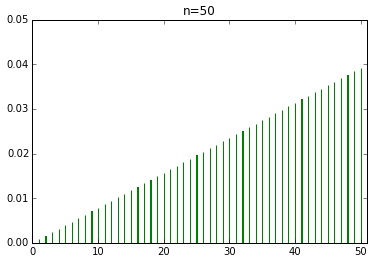
\includegraphics[scale=.6]{./images/3e_pmf-line_graph.png}
	    % 3e_pmf-line_graph.png: 384x262 pixel, 96dpi, 10.16x6.93 cm, bb=0 0 288 196
	  \end{figure}
	  
	%f
	\item
	  \begin{align*}
	   1 &= \mathlarger{\sum}_{x=0}^\infty{\dfrac{c}{(x+1)(x+2)}} \\
	     &= c \mathlarger{\sum}_{x=0}^\infty{\dfrac{1}{(x+1)(x+2)}} \\
	     &= c \mathlarger{\sum}_{x=0}^\infty{\left(\dfrac{1}{x+1} - \dfrac{1}{x+2}\right)} \\
	     &= c \left[ \left( \dfrac{1}{1} - \dfrac{1}{2} \right) 
		  + \left( \dfrac{1}{2} - \dfrac{1}{3} \right)  
		  + \left( \dfrac{1}{3} - \dfrac{1}{4} \right) + \cdots \right] \\
	     &= c (1)
	  \end{align*}
	  
	  Therefore, $c = 1$.
	  
	  \begin{figure}[h!]
	    \centering
	    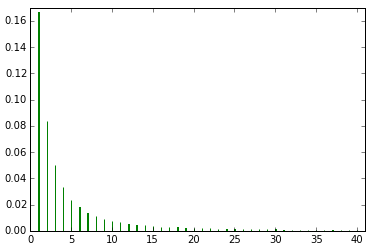
\includegraphics[scale=.6]{./images/3f_pmf-line_graph.png}
	    % 3f_pmf-line_graph.png: 378x251 pixel, 96dpi, 10.00x6.64 cm, bb=0 0 283 188
	  \end{figure}

      \end{enumerate}
      
     %4 
     \item
      \begin{enumerate}
	%a
	\item 
	  The pmf of X for true random numbers is $f(x) = P(X = x) = \dfrac{1}{10}$ for $x=0,1,2,\dots,9$.
	  
	  \begin{figure}[h!]
	    \centering
	    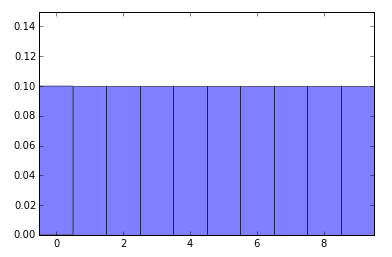
\includegraphics[scale=.7]{./images/4a_probabilityHistogram.png}
	    % 4a_probabilityHistogram.png: 392x257 pixel, 96dpi, 10.37x6.80 cm, bb=0 0 294 193
	  \end{figure}

	\newpage
	%b
	\item
	  Relative frequencies of integers
	  \begin{longtable}[c]{@{}lc@{}}
	    \toprule
	    Integer & Relative Frequency\tabularnewline
	    \midrule
	    \endhead
	    0 & 11/150 (.0733) \tabularnewline
	    1 & 14/150 (.0933) \tabularnewline
	    2 & 13/150 (.0867) \tabularnewline
	    3 & 12/150 (.0800) \tabularnewline
	    4 & 16/150 (.1067) \tabularnewline
	    5 & 13/150 (.0867) \tabularnewline
	    6 & 22/150 (.1467) \tabularnewline
	    7 & 16/150 (.1067) \tabularnewline
	    8 & 18/150 (.1200) \tabularnewline
	    9 & 15/150 (.1000) \tabularnewline
	    \bottomrule
	  \end{longtable}
	  
	%c
	\item
	  Relative frequencies histogram in red dotted line over probability histogram:
	  
	  \begin{figure}[h!]
	    \centering
	    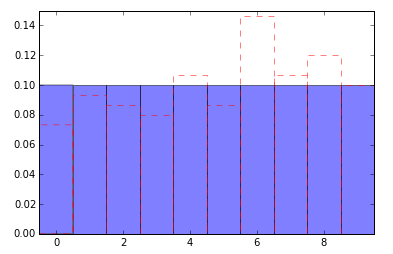
\includegraphics[scale=.7]{./images/4c_probabilityHistogram-and-relativeFrequencies.png}
	    % 4c_probabilityHistogram-and-relativeFrequencies.png: 393x254 pixel, 96dpi, 10.40x6.72 cm, bb=0 0 295 190
	  \end{figure}
      \end{enumerate}

     \addtocounter{enumi}{4}
     
     %9
     \item 
      $f(x) = \dfrac{(1 + |x - 3|)}{11}$
      \begin{figure}[h!]
	\centering
	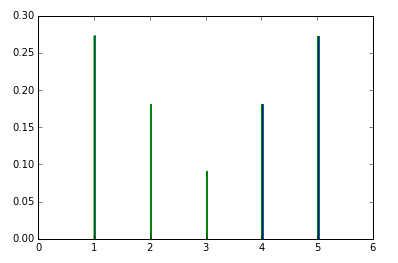
\includegraphics[scale=.7]{./images/9_pmf-line_graph.png}
	% 9_pmf-line_graph.png: 398x263 pixel, 96dpi, 10.53x6.96 cm, bb=0 0 298 197
      \end{figure}

      
     %10
     \item 
      \begin{enumerate}
       %a
       \item 
	  $P(X = 1) = \dfrac{\dbinom{3}{1}\dbinom{47}{9}}{\dbinom{50}{10}} = 0.3980$
	  
       %b
       \item
	  $P(X \le 1) = P(X = 0) + P(X = 1) = 
	    \dfrac{\dbinom{3}{0}\dbinom{47}{10}}{\dbinom{50}{10}} +
	    \dfrac{\dbinom{3}{1}\dbinom{47}{9}}{\dbinom{50}{10}} = 0.5041 + 0.3980 = 0.9021$
      \end{enumerate}

     %11
     \item
	\begin{align*}
	  P(X \ge 1) &= 1 - P(X < 1) \\
		     &= 1 - P(X = 0) \\
		     &= 1 - \dfrac{\dbinom{5}{0}\dbinom{95}{10}}{\dbinom{100}{10}} \\
		     &= 1 - 0.5838 \\
		     &= 0.4162
	\end{align*}
    \end{enumerate}
    
    Section 2.2
    \begin{enumerate}
     %1
     \item 
      \begin{enumerate}
       %a
       \item 
	  $E(X) = \mathlarger{\sum}_{x=1}^4{x\dfrac{x}{10}} = \dfrac{1}{10}[1^2+2^2+3^2+4^2] = 3$
       %b
       \item 
	  $E(X) = \mathlarger{\sum}_{x=1}^{10}{x\dfrac{x}{55}} = \dfrac{1}{55}[1^2+2^2+\cdots+10^2]
	    = \dfrac{385}{55} = 7$
       
       %c
       \item
	  \begin{align*}
	    E(X) - \dfrac{1}{4}E(X) 
	      &= \mathlarger{\sum}_{x=1}^\infty{x\cdot3\left(\dfrac{1}{4}\right)^x} 
	      - \mathlarger{\sum}_{x=1}^\infty{x\left(\dfrac{1}{4}\right)3\left(\dfrac{1}{4}\right)^x} \\
	    \dfrac{3}{4}E(X) &= \left[3(1)\left(\dfrac{1}{4}\right)^1 + 3(2)\left(\dfrac{1}{4}\right)^2
		+ 3(3)\left(\dfrac{1}{4}\right)^3 + \cdots \right] - \\
		& \left[ 3(1)\left(\dfrac{1}{4}\right)\left(\dfrac{1}{4}\right)^1 +
		3(2)\left(\dfrac{1}{4}\right)\left(\dfrac{1}{4}\right)^2 +
		3(3)\left(\dfrac{1}{4}\right)\left(\dfrac{1}{4}\right)^3 + \cdots \right] \\
	    &= 3 \left\{ \left[ 1\left(\dfrac{1}{4}\right)^1 + 2\left(\dfrac{1}{4}\right)^2
		+ 3\left(\dfrac{1}{4}\right)^3 + \cdots \right] -
		\left[ 1\left(\dfrac{1}{4}\right)^2
		+ 2\left(\dfrac{1}{4}\right)^3 + 3\left(\dfrac{1}{4}\right)^4 + \cdots \right] \right\} \\
	    &= 3 \left[ 1 \left(\dfrac{1}{4}\right)^1 + 1 \left(\dfrac{1}{4}\right)^2
		+ 1 \left(\dfrac{1}{4}\right)^3 + \cdots \right] \\
	    &= 3 \left( \dfrac{1}{3} \right) = 1
	  \end{align*}
	  
	  Therefore, $E(X) = \dfrac{4}{3}$
	  
       %d
       \item
	  \begin{align*}
	   E(X) &= \mathlarger{\sum}_{x=0}^3{x\dfrac{(x+1)^2}{30}} \\
	      &= 0\left(\dfrac{(0+1)^2}{30}\right) + 1\left(\dfrac{(1+1)^2}{30}\right) 
		+ 2\left(\dfrac{(2+1)^2}{30}\right) + 3\left(\dfrac{(3+1)^2}{30}\right) \\
	      &= 0 + \dfrac{4}{30} + \dfrac{18}{30} + \dfrac{48}{30} \\
	      &= \dfrac{70}{30} = \dfrac{7}{3}
	  \end{align*}
	  
       %e
       \item
	  \begin{align*}
	   E(X) &= \mathlarger{\sum}_{x=1}^n{x\cdot \dfrac{x}{\dfrac{n(n+1)}{2}}}
		  = \mathlarger{\sum}_{x=1}^n{\dfrac{2x^2}{n(n+1)}} \\
	      &= \left[ \dfrac{2(1)^2}{n(n+1)} + \dfrac{2(2)^2}{n(n+1)} + \dfrac{2(3)^2}{n(n+1)} +
		  \cdots + \dfrac{2n^2}{n(n+1)} \right] \\
	      &= 2 \left[ \dfrac{n(n+1)(2n+1)}{6n(n+1)} \right] \\
	      &= \dfrac{2n+1}{3}
	  \end{align*}
	  
       %f
       \item
	  \begin{align*}
	   E(X) &= \mathlarger{\sum}_{x=0}^\infty{x \cdot \dfrac{1}{(x+1)(x+2)}} \\
	      &= \mathlarger{\sum}_{x=0}^\infty{x\left(\dfrac{1}{x+1}-\dfrac{1}{x+2}\right)} \\
	      &= \left[ 0\left(\dfrac{1}{1} - \dfrac{1}{2}\right) + 
		  1\left(\dfrac{1}{2} - \dfrac{1}{3}\right) + 2\left(\dfrac{1}{3} - \dfrac{1}{4}\right)
		  + 3\left(\dfrac{1}{4} - \dfrac{1}{5}\right) + \cdots \right] \\
	      &= \left[ 0 + \dfrac{1}{2} + \dfrac{1}{3} + \dfrac{1}{4} + \cdots \right] \\
	      &= \mathlarger{\sum}_{x=2}^\infty{\dfrac{1}{x}}
	  \end{align*}
	  
	  The sum $\mathlarger{\sum}_{x=2}^\infty{\dfrac{1}{x}}$ does not converge to a finite
	value. Therefore $E(X)$ does not exist.

      \end{enumerate}

     %2
     \item 
	\begin{align*}
	 E(X) &= \mathlarger{\sum}_{x = -1}^1{x \cdot \dfrac{(|x| + 1)^2}{9}} \\
	    &= (-1)\left(\dfrac{(|-1| + 1)^2}{9}\right) + (0)\left(\dfrac{(|0|+ 1)^2}{9}\right)
		+ (1)\left(\dfrac{(|1| + 1)^2}{9}\right) \\
	    &= -\dfrac{4}{9} + 0 + \dfrac{4}{9} \\
	    &= 0
	\end{align*}
	
	\begin{align*}
	 E(X^2) &= \mathlarger{\sum}_{x = -1}^1{x^2 \cdot \dfrac{(|x| + 1)^2}{9}} \\
	    &= (-1)^2\left(\dfrac{(|-1| + 1)^2}{9}\right) + (0)^2\left(\dfrac{(|0|+ 1)^2}{9}\right)
		+ (1)^2\left(\dfrac{(|1| + 1)^2}{9}\right) \\
	    &= \dfrac{4}{9} + 0 + \dfrac{4}{9} \\
	    &= \dfrac{8}{9}
	\end{align*}
	
	\begin{align*}
	 E(3X^2 - 2X + 4) &= 3E(X^2) - 2E(X) + 4 \\
			  &= 3\left(\dfrac{8}{9}\right) - 2(0) + 4 \\
			  &= \dfrac{8}{3} + 4 \\
			  &= \dfrac{20}{3}
	\end{align*}
      \addtocounter{enumi}{1}
      
     %4
     \item
	\begin{align*}
	 0.1 &= \mathlarger{\sum}_{x=1}^6{\dfrac{c}{x}} \\
	     &= \left( \dfrac{c}{1} + \dfrac{c}{2} + \dfrac{c}{3} + \dfrac{c}{4} + \dfrac{c}{5}
		+ \dfrac{c}{6} \right) \\
	     &= \dfrac{147c}{60} = \dfrac{49c}{20}
	\end{align*}
	
	Therefore, $c = \dfrac{2}{49}$
	
	\begin{align*}
	 E(X) &= \mathlarger{\sum}_{x=1}^6{x\cdot \dfrac{2}{49x}} 
		= \mathlarger{\sum}_{x=1}^6{\dfrac{2}{49}} \\
	      &= 6\cdot \dfrac{2}{49} \\
	      &= \dfrac{12}{49}
	\end{align*}
	
	Subtracting 1 for the deductible: 
	$$E(X) - 1 = \dfrac{12}{49} - \dfrac{49}{49} = -\dfrac{37}{49}$$
	
     %5
     \item 
	\begin{enumerate}
	 %a
	 \item 
	    pmf of Z, $h(z) = \dfrac{(4 - \sqrt[3]{z})}{6}$ for $z=1,8,27$
	    
	 %b
	 \item
	    $E(Z) = (1)\left(\dfrac{3}{6}\right) + (8)\left(\dfrac{2}{6}\right) 
		    + (27)\left(\dfrac{1}{6}\right) = \dfrac{46}{6} = \dfrac{23}{3}$
	
	 %c
	 \item
	    He can expect to make $10 - \dfrac{23}{3} = \dfrac{7}{3}$ of a dollar on the average
	    each play.
	\end{enumerate}

     %6
     \item
	\begin{align*}
	 E(X) &= \mathlarger{\sum}_{x=1}^\infty{x\cdot \dfrac{6}{\pi^2 x^2}} \\
	      &= \dfrac{6}{\pi^2} \mathlarger{\sum}_{x=1}^\infty{\dfrac{1}{x}}
	\end{align*}

	The sum $\mathlarger{\sum}_{x=1}^\infty{\dfrac{1}{x}}$ does not converge to a finite
	value. Therefore $E(X)$ does not exist.
     \addtocounter{enumi}{2}
     
     %9
     \item
	\begin{enumerate}
	 %a
	 \item 
	    $E(X) = (-1)\left(\dfrac{20}{38}\right) + (1)\left(\dfrac{18}{38}\right) = -\dfrac{1}{19}$
	    
	 %b
	 \item
	    $E(X) = (-1)\left(\dfrac{19}{37}\right) + (1)\left(\dfrac{18}{37}\right) = -\dfrac{1}{37}$
	\end{enumerate}
     \addtocounter{enumi}{2}
	
     %12
     \item
	\begin{enumerate}
	 %a
	 \item 
	    Average class size: $\dfrac{16(25) + 3(100) + 1(300)}{20} = \dfrac{1000}{20} = 50$
	  
	 %b
	 \item
	    pmf of X:
	    
	    \[  f(x) = 	    
		\begin{cases}
	         \hfill \frac{16}{20} \hfill & x=25, \\
	         \hfill \frac{3}{20}  \hfill & x=100, \\
	         \hfill \frac{1}{20}  \hfill & x=300, \\
	         \hfill 0	      \hfill & \text{all other x} \\
	        \end{cases} \]	    
	    
	 %c
	 \item
	    $E(X) = (25)\left(\dfrac{16}{20}\right) + (100)\left(\dfrac{3}{20}\right)
		    + (300)\left(\dfrac{1}{20}\right) = 50$
		    
	    No, this answer does not surprise me.
	\end{enumerate}

      
    \end{enumerate}

\end{document}